%_________Einleitung__________________________________
\chapter{Introduction}
\begin{figure}[H]
	\centering
	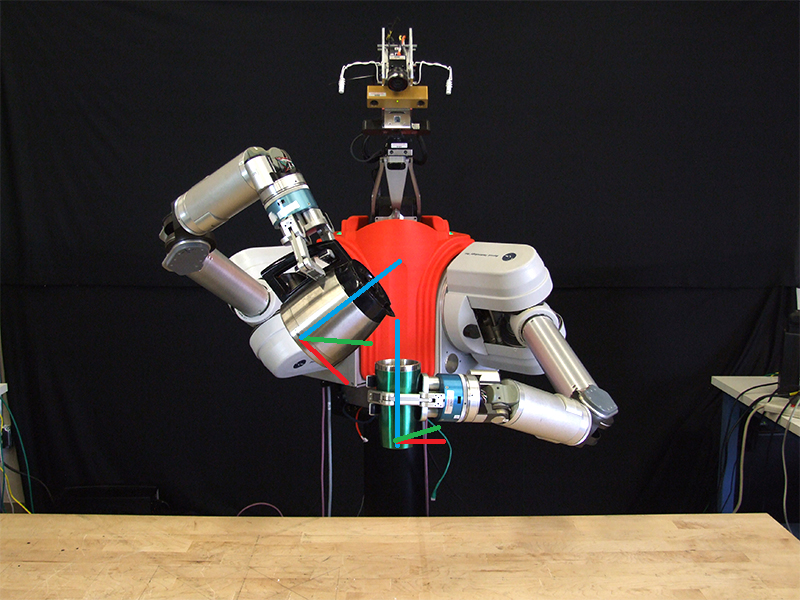
\includegraphics[width=0.75\textwidth]{intro}
	\caption[Example of object pose estimation application.]{\textbf{Example of object pose estimation application.}}
	\label{fig:intro}
\end{figure}

Fueled by the developments in robotics, autonomous driving and augmented/mixed reality, object pose estimation has become a popular research trend in computer vision. Although many encouraging achievements have emerged in recent years, a reliable and fast pose estimation still remains as an open challenge. The main deficiencies of the existing methods are (\romannumeral 1) not robust enough against object occlusions, background clutter and dynamic environment; (\romannumeral 2) often require object to have certain properties such as enough textual surface structure and asymmetric shape; (\romannumeral 3) not efficient to run in real time; (\romannumeral 4) often require a big amount of annotated training data.    
\\[8pt]
In order to conquer the above-mentioned challenges, a novel deep-learning-based approach is presented in \cite{sundermeyer2018implicit}, which operates on single RGB images and yield a fast and robust estimation in different scenarios.
\\[8pt]
In this project, I implemented the approach proposed in \cite{sundermeyer2018implicit}. I firstly generated a synthetic dataset with textured mesh model \cite{calli2015ycb}, and then trained an aotoencoder on the generated dataset. After training, I abstracted useful features from images using the autoencoder, and finally estimated the pose of the object through nearest neighbor search.
